\newpage
\section{Aufgabenstellung 1 Taucher}

%% Gruppengröße die bereits geformten Teams
%% Alle verwendeten Quellen sind anzugeben.
%% Abzugeben bis zum 04.05.2025 um 23:59 Uhr
%% Abgabe = ein PDF-Dokument der gesamten Gruppe in folgendem Schema
                      
%%   SS2025_DevOps_ILV_Gruppe_[Gruppenbuchstabe]_Aufgabe_1 beispielsweise
%%   240223_DevOps_ILV_Gruppe_A_Aufgabe_1 für die Gruppe A

%% Bei Fragen kontaktiert mich gerne per E-Mail: stefan.taucher@fh-burgenland.at
%% Aufgabenstellung siehe Datei  Aufgabe.pdf .

\subsection{Teilbereich Build and Code}
Die Agile Softwareentwicklung in der Art und Weise wie Sie heute praktiziert und rezitiert wird, basiert auf dem Manifest für Agile Softwareentwicklung. 
Agile Software Entwicklung setzt sich aus an Agilität ausgerichteten Methoden und agilen Prozessen zusammen. 

% Please add the following required packages to your document preamble:
% \usepackage{graphicx}
\subsubsection{Vorgehensmodelle}
Aufbauend auf das agile Manifest haben sich eine Vielzahl von Frameworks für das Management der agilen Prozesse entwickelt. 
Diese sind mit Fokus auf die Software Entwicklung entstanden, haben aber ihren Weg auch schon in andere Bereiche angetreten. 
Einige ausgewählte Frameworks sollen nachfolgenden kurz präsentiert werden. 
\newline
\begin{table}[h!]
    \centering
    \caption{Agile Prozessmanagement Frameworks der Software Entwicklung}
    \label{tab:agile-frameworks}
    \begin{tabular}{|l|l|}
    \hline
    \textbf{Framework}            & \textbf{Abkürzung} \\ \hline
    Extreme Programming           & XP                 \\ \hline
    Feature Driven Development    & FDD                \\ \hline
    Kanban in der IT              & IT-Kanban          \\ \hline
    Adaptive Software Development & ASD                \\ \hline
    Crystal Family                & CF                 \\ \hline
    Agile unified process         & AUP                \\ \hline
    Lean software development     & LSD                \\ \hline
    Large Scale Agile Frameworks  & LSAF               \\ \hline
    \end{tabular}
\end{table} 
\newline
Die Leitwerte des \textbf{XP} sind Kommunikation, Einfachheit, Feedback und Mut und sollen durch die Praktiken:
Vor-Ort-Kunde, Planspiel, Metapher, einfaches Design, kleines Release, Pair Programming, Testen, Refactoring, 
kontinuierliche Integration, 40-Stunden-Woche, Coding Standard und kollektive Verantwortung für die Entstehung 
eines optimalen Produktes sorgen. Einige dieser Praktiken bzw. Methoden werden auch in anderen agilen Frameworks 
genutzt, im XP wird aber stark auf die Synergieeffekte zwischen den Leitwerten und Praktiken wert gelegt. \cite{FOJTIK20111464}
\newline Mohammad Alshayeb und Wie Li untersuchten die spezifischen Praktiken und stellten im XP folgende Tätigkeiten
als Hauptaktivitäten der Entwickler fest: Refactoring, neues Design, Beheben von Fehlern und Implementieren von Unit- 
sowie Funktionstests, um die Funktionstüchtigkeit des Produktes sicherzustellen. \cite{Alshayeb2006-nt}
\newline
Das \textbf{FDD} hat sich aus der Coad Methode von Peter Coad entwickelt und besteht nur aus zwei Hauptphasen. 
Der Entdeckungsphase und der Implementierungsphase. Hauptaugenmerk wird dabei auf die Entdeckungsphase gelegt, da hier sowohl die Liste der Features erstellt wird, als auch die UML-Diagramme der spezifischen Kundendomäne. 
Die Mitwirkung des Kunden ist besonders wichtig, damit die Wartbarkeit und Erweiterbarkeit des Codes im weiteren Projektverlauf gewährleistet werden kann. 
Die verwendete Sprache sollte von sowohl von Entwickler:innen, als auch von Kundenseite verstanden werden. \cite{Chowdhury2011-hg}
\newline
\textbf{Kanban} ist eine Methodik aus der Produktionsindustrie und wurde von Mary und Tom Poppenieck und später von David Anderson für 
die Software Entwicklung adaptiert. Im Gegensatz zu den meisten anderen agilen Frameworks gibt es keine spezifischen Arbeitsabläufe, 
Rollen oder zeitliche Begrenzungen des Arbeitsprozesses in Iterationen. 
Hauptaufgabe ist es, den Arbeitsfluss zu koordinieren und in Teilaufgaben zu unterteilen. Anderson beschreibt dazu fünf Kernprinzipien für IT-Kanban:
\begin{itemize}
    \item Arbeitsablauf visualisieren
    \item Arbeit, die noch nicht abgeschlossen ist, begrenzen des Work in Progress (WIP) 
    \item Arbeitsfluss messen und verwalten
    \item Richtlinien für den Arbeitsprozess definieren und explizit sichtbar machen
    \item Nutzung von Modellen aus der Praxis oder Theorie, um Verbesserungsmöglichkeiten im Arbeitsablauf zu erkennen.
\end{itemize}
Die Visualisierung erfolgt durch das sogenannte Kanban-Board, das sowohl die Begrenzung der Arbeitslast bzw. des Arbeitspakets, 
als auch die Priorisierung der Aufgabe und das Eingreifen bei Engpässen im Arbeitsfluss ermöglicht. \cite{Ahmad2018-jv,Granulo2019-wm}
\newline
In \textbf{ASD} wird der Fokus auf ein zyklisches Weiterentwicklungsmodell gelegt, das die unterschiedlichen Phasen im Lebenszyklus
der Software widerspiegelt. \cite{Abdelaziz2015-lb}
\begin{figure}[h!]
\centering
\caption{ASD-Diagramm}
    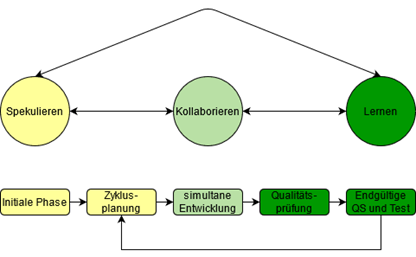
\includegraphics[width=0.5\textwidth]{fig/ASD.png}
    \label{fig:ASD-diagram}
\end{figure}
\begin{itemize}
    \item \textbf{Spekulieren:} ersetzt planen, um hier mehr Raum für Innovation und Ungewissheit bei komplexen Problemen zu schaffen.
    \item \textbf{Kollaborieren/Zusammenarbeiten:} Bei komplexen Software-Anwendungen und sich ändernden Anforderungen ist der Informationsfluss nur durch die Zusammenarbeit im Team schaffbar.
    \item \textbf{Lernen:} In dieser Phase können die technischen Parameter und Kundenwünsche regelmäßig nach den abgeschlossenen einzelnen Iterationen überprüft werden
\end{itemize}
\cite{Alnoukari2008-ro,Abdelaziz2015-lb}
\newline
Die \textbf{CF} wurde von Alistair Cockburn erstellt, um im Rahmen der Entwicklung von Software, ähnlich wie bei einem Kristall oder Edelstein, 
je nach Größe des Projektes unterschiedliche Methoden, Techniken und Richtlinien nutzen zu können. Die Methoden fokussieren sich 
dabei auf folgende Parameter \cite{Ibrahim2020-ip}:
\begin{itemize}
    \item \textbf{Menschen}
    \item \textbf{Interaktionen} 
    \item \textbf{Gemeinschaft}    
    \item \textbf{Fertigkeiten}
    \item \textbf{Talente und Kommunikation }
\end{itemize}
Die Methoden von Crystal werden nach Farben benannt und nach der Größe des Projektes und der Anzahl der Projektmitarbeiter*Innen eingeteilt.
\begin{figure}
    \centering
    \caption{CS-Diagramm}
        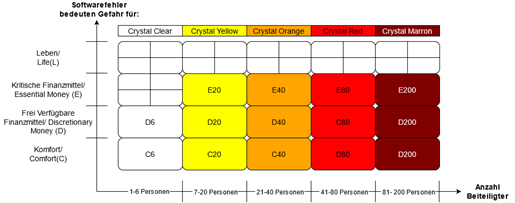
\includegraphics[width=0.5\textwidth]{fig/CSD.png}
        \label{fig:CS-diagram}
    \end{figure}
Auf der Y-Achse werden die vier Level des Gefahrenlevels definiert und auf der X-Achse die Anzahl der Beteiligten. 
Hier angezeigt werden die Crystal Methoden, die noch nicht das Risikolevel Leben abdecken können. 
Crystal Clear sollen Projekte mit fixiertem Preis und klaren Parameter sein und sobald Projekte Gefahr für Leib 
und Leben beinhalten, handelt es sich dabei um Crystal Diamond und Crystal Sapphire.\cite{cockburn2004,Ibrahim2020-ip}
\newline
\textbf{AUP} ist ein Framework bzw. Modellierungsansatz, der von Scott Ambler aus dem Rational Unified Process (RUP) mit agilen Methoden kombiniert entwickelt wurde. 
Ambler definiert dafür folgende Kernprinzipen \cite{Christou2010-vf}:
\begin{itemize}
    \item Die meisten Menschen werden keine detaillierte Dokumentation lesen.  Sie werden jedoch hin und wieder Anleitung und Schulung benötigen
    \item Das Projekt sollte einfach mit wenigen Seiten beschrieben werden.
    \item Die AUP entspricht den von der Agile Alliance beschriebenen Werten und Prinzipien.    
    \item Das Projekt muss sich darauf konzentrieren, einen wesentlichen Wert zu liefern und nicht unnötige Funktionen.
    \item Die Entwickler müssen die Freiheit haben, Werkzeuge zu verwenden, die für die jewei-lige Aufgabe am besten geeignet sind, und nicht, um eine Vorschrift zu erfüllen.
    \item AUP lässt sich über gängige HTML-Editierwerkzeuge leicht anpassen. 
\end{itemize}
Es werden dann vier seriell ablaufende Phasen definiert \cite{Li2010-ge,ShuiYuan2009-or}:
\begin{itemize}
    \item \textbf{Inception/Beginn}: Ziel ist es, den anfänglichen Umfang des Projekts und eine potenzielle Architektur für Ihr System festzulegen, sowie die anfängliche Projektfinanzierung und die Akzeptanz der Stakeholder zu erhalten.
    \item \textbf{Elaboration/Ausarbeitung:} Die Architektur des Systems wird überprüft.
    \item \textbf{Construction/Konstruktion: }Es soll regelmäßig und schrittweise funktionierende Software erstellt werden, welche die Anforderungen der Projektbeteiligten mit höchster Priorität erfüllt.
    \item \textbf{Transition/Übergabe:} Das Ziel ist die Validierung und der Einsatz ihres Systems in ihrer Produktionsumgebung
\end{itemize}

LSD hat als Vorbild das Toyota Produktionssystem und definiert sieben Prinzipien und 22 Praktiken für die Umsetzung im Rahmen der agilen Softwareentwicklung. 
Die sieben Prinzipien sind \cite{Janes2015-ir,Jonsson2013-gn}:
\begin{itemize}
    \item Verschwendung vermeiden
    \item Lernen unterstützen
    \item So spät entscheiden wie möglich
    \item Verantwortung an das Team geben
    \item Integrität einbauen
    \item Das Ganze sehen
\end{itemize}
Unterschiedliche \textbf{LSAF}  sind entwickelt worden, um agile Praktiken auf große Projekte und Softwareentwicklung 
mit weltweit verteilten Teams anzuwenden. Zu den bekanntesten Modellen zählen\cite{Beecham2021-jj,Ebert2017-jz}:
\begin{itemize}
    \item \textbf{Scrum of Scrums (SoS)}
    \item \textbf{Scaled Agile Framework (SAFe)} 
    \item \textbf{Large-Scale Scrum (LeSS)}    
    \item \textbf{Disciplined Agile Delivery (DAD)}
    \item \textbf{Lean Scalable Agility for Engineering (LeanSAFE)}
\end{itemize}
Kieran Conboy und Noel Carroll definieren ausgehend von einer 15-jährigen Retrospektive folgende Herausforderungen bei der
Implementation von Large Scale Agile Frameworks \cite{Conboy2019-uw,Kasauli2021-jn}:
\begin{itemize}
    \item Definieren von Konzepten
    \item Vergleich und Gegenüberstellung von Frameworks
    \item Bereitschaft und Appetit auf Veränderung
    \item Abgleich von Organisationsstruktur und Rahmenbedingungen
    \item Top-down- versus Bottom-up-Implementierung
    \item Überbetonung der 100 \%igen Einhaltung der Regeln des Frameworks gegenüber dem Mehrwert für die Firma
    \item Fehlender evidenzbasierter Einsatz
    \item Erhaltung der Autonomie der Entwickler und Entwicklerteams
    \item Fehlende Abstimmung zwischen Kundenprozessen und Frameworks
\end{itemize}

\textbf{Fragestellung:} Welche bereits vorgestellten bzw. zusätzlich recherchierte Vorgehensmodelle ermöglichen ein
schnelles Iterieren und somit die Möglichkeit Feedback zeitnah durch die jeweiligen Stakeholder
einzubringen? Zusätzlich soll auch darauf eingegangen werden, weshalb die gewählten
Vorgehensmodelle dies im Vergleich zu anderen Modellen ermöglichen.
\\

\paragraph{Scrum}



\paragraph{Extreme Programming}


\paragraph{Test-Driven Development}


\paragraph{Kanban}



\subsubsection{Extreme Programming}

\textbf{Fragestellung:} Beschreiben Sie mindestens 3 Praktiken aus Extreme Programming im Detail und den Einfluss
die diese Praktik auf die Softwareentwicklung und dem Ergebnis haben.

\paragraph{Pair Programming}
Beim Pair Programming arbeiten zwei Entwickler gemeinsam an einem Computer. Eine Person (der Driver) schreibt den Code, 
während die andere Person (der Navigator) den Code überprüft, Probleme identifiziert und strategische Entscheidungen trifft. 
Die Rollen werden regelmäßig gewechselt.

\textbf{Einfluss auf die Softwareentwicklung:}
\begin{itemize}
    \item \textbf{Verbesserte Codequalität:} Durch kontinuierliches Review werden Fehler früher erkannt und behoben.
    \item \textbf{Wissenstransfer:} Entwickler lernen voneinander, was zu einer breiteren Verteilung von Wissen im Team führt.
    \item \textbf{Bessere Lösungsansätze:} Durch die Kombination verschiedener Perspektiven entstehen oft kreativere und effizientere Lösungen.
    \item \textbf{Reduzierte technische Schulden:} Die kontinuierliche Überprüfung verhindert Abkürzungen und schlechte Praktiken.
\end{itemize}

\paragraph{Continuous Integration (CI)}
Bei der Continuous Integration werden Codeänderungen mehrmals täglich in ein gemeinsames Repository integriert. Nach jeder Integration 
werden automatisierte Tests durchgeführt, um sicherzustellen, dass die Änderungen keine Fehler verursachen.

\textbf{Einfluss auf die Softwareentwicklung:}
\begin{itemize}
    \item \textbf{Frühe Fehlererkennung:} Probleme werden unmittelbar nach ihrer Entstehung identifiziert, was die Behebungskosten drastisch reduziert.
    \item \textbf{Reduzierte Integrationszeit:} Durch häufige kleine Integrationen werden große, problematische Merges vermieden.
    \item \textbf{Höhere Softwarestabilität:} Die Software bleibt kontinuierlich in einem funktionsfähigen Zustand.
    \item \textbf{Schnelleres Feedback:} Entwickler erhalten unmittelbare Rückmeldung zu ihren Änderungen.
\end{itemize}

\paragraph{Test-Driven Development (TDD)}
Bei TDD werden Tests geschrieben, bevor der eigentliche Code implementiert wird. Der Entwicklungsprozess folgt 
einem Red-Green-Refactor-Zyklus: Zuerst wird ein fehlschlagender Test geschrieben (Red), dann wird gerade genug Code implementiert,
um den Test zu bestehen (Green), und schließlich wird der Code verbessert, ohne seine Funktionalität zu ändern (Refactor).

\textbf{Einfluss auf die Softwareentwicklung:}
\begin{itemize}
    \item \textbf{Klarere Anforderungen:} Das Schreiben von Tests zwingt Entwickler, die Anforderungen genau zu verstehen.
    \item \textbf{Besseres Design:} TDD fördert modularen, entkoppelten Code, der leichter zu testen ist.
    \item \textbf{Umfassende Testabdeckung:} Jede Funktionalität wird durch Tests abgedeckt, was zu robusterer Software führt.
    \item \textbf{Dokumentation durch Tests:} Tests dienen als lebende Dokumentation, die zeigt, wie der Code verwendet werden soll.
    \item \textbf{Sicherheit bei Refactoring:} Entwickler können Code mit Vertrauen umgestalten, da Tests Regressionen aufdecken.
\end{itemize}

    %% possibile quellens:
    %% https://www.it-agile.de/agiles-wissen/agile-entwicklung/was-ist-extreme-programming/
    %% https://www.agile-heroes.com/de/magazine/extreme-programming/
    %% https://asana.com/de/resources/extreme-programming-xp


\subsubsection{Zusammenfassung von Artikel Spotify Scaling}

Aufgabenstellung:Lesen Sie den Artikel https://blog.crisp.se/wp-content/uploads/2012/11/SpotifyScaling.pdf.
Diese Informationen fassen Sie bitte in 1 bis maximal 2 Seiten zusammen


\subsubsection{Git Features}

Fragestellung: Beschreiben Sie Git im Detail sowie mindestens 2 Features im Detail.

\paragraph{Was ist Git?}
Git ist ein verteiltes Versionskontrollsystem, das 2005 von Linus Torvalds entwickelt wurde.
Es ermöglicht die Verwaltung von Änderungen an Dateien und Projekten,
wobei jeder Entwickler eine vollständige Kopie des Projekts und seiner Historie auf seinem lokalen System hat.
Git ist besonders für seine Geschwindigkeit, Datenintegrität und Unterstützung für nicht-lineare, verteilte Workflows bekannt \cite{github-git}.

\paragraph{Feature 1: Branching und Merging}
Git bietet ein leistungsfähiges Branching-System, das es ermöglicht, parallele Entwicklungslinien zu erstellen und zu verwalten.
Branches sind leichtgewichtige Zeiger auf einen bestimmten Commit. Entwickler können schnell neue Branches erstellen,
zwischen ihnen wechseln und sie zusammenführen. Dies ermöglicht:

    \begin{itemize}
        \item Isolierte Entwicklung neuer Features
        \item Experimentieren ohne Risiko für den Hauptcode
        \item Parallele Arbeit an verschiedenen Aspekten des Projekts
        \item Einfaches Zusammenführen von Änderungen durch Merging
    \end{itemize}

    \paragraph{Feature 2: Distributed Version Control}
    Git ist ein vollständig verteiltes System, was bedeutet, dass jeder Entwickler eine vollständige Kopie des Repositories besitzt.
    Dies bietet mehrere Vorteile:

    \begin{itemize}
        \item Offline-Arbeit ist möglich
        \item Schnelle Operationen durch lokale Ausführung
        \item Redundanz und Backup durch multiple Kopien
        \item Flexible Workflow-Möglichkeiten
        \item Keine zentrale Schwachstelle
    \end{itemize}




    %% possibile quellens:
    %% https://docs.github.com/en/get-started/using-git/about-git
    %% https://www.geeksforgeeks.org/git-features/
    %% https://www.simplilearn.com/tutorials/git-tutorial/what-is-git#features_of_git


\subsubsection{Qualitätssteigernde Maßnahmen}

Fragestellung: Welche qualitätssteigenden Maßnahmen kennen Sie? Beschreiben Sie 2 beliebige im Detail.

   %% possibile quellens:
    %% code review https://about.gitlab.com/topics/version-control/what-is-code-review/
    %% automated testing https://www.testdevlab.com/blog/automated-testing
    %% weitere Bsp wären Continuous Integration/Continuous Deployment (CI/CD), Code Standards, 
    %% Logging, Code Refactoring 


\subsection{Teilbereich DevOps}

\subsubsection{Aufgabenstellung}

Das Unternehmen ABC Ad Tech stellt eine SaaS-Lösung für Kunden bereit mit denen ihre
Werbekampagnen verwaltet werden können.
Aktuell gibt es ein Entwicklungsteam namens  Ad-Dev  mit 5 Personen die gemeinsam die
Lösung entwickeln. Der Source Code ist hierzu in git abgelegt. Der Output des Build-Prozesses
(=Artefakt) wird auf dem Firmen-PC von einem speziellen Mitarbeiter erstellt und dann
händisch auf eine Netzwerkdateifreigabe kopiert.
Für die Kunden wird die Lösung aktuell durch das Team namens Ad-Ops betrieben.
Die beiden Teams arbeiten unabhängig voneinander.
Das Entwicklungsteam Ad-Dev liefert alle 3 Monate eine neue Produktivversion und alle
zwei Woche eine neue Testversion. Beide werden von Team Ad-Ops bei Verfügbarkeit
eingespielt, d.h. es wird das Artefakt von der Netzwerkdateifreigabe herunterkopiert und dann
händisch eingespielt. Die Testversion kommt immer auf eine Staging-Umgebung, welche
vom Team Ad-QS getestet wird und anschließend wird das Feedback mittels einer
Besprechung an die Entwicklung rückgemeldet. Auch die Produktivversion wird zuerst auf der
Staging-Umgebung getestet und sobald die Freigabe seitens  Ad-QS  gegeben wird erfolgt die
Einspielung auf das Produktivsystem durch das Team Ad-Ops. Bei Problemen und sonstigen
Auffälligkeiten wird vom Team  Ad-Ops  aus Kontakt mit dem Entwicklungsteam  Ad-Dev 
aufgenommen.\\


\subsubsection{Mögliche Probleme in der aktuellen Organisation und Arbeitsaufteilung}

\textbf{Fragestellung:} Beschreibe kurz mögliche Probleme in der aktuellen Organisation und Arbeitsaufteilung
    
%% mögliche Problems:
%% Manuelles deployn -- Fehleranfällig -- Mensch 
%% devs und ops arbeiten unabhängig voneinander - keine Kommunikation
%% Probleme werden erst adressiert wenn sie zufällig gefunden werden - kein Monitoring
%% alle 3 Monate wird ausgeliefert - keine Continuous Delivery

\subsubsection{Notwendige Schritte um in dieser Organisation DevOps einzuführen}
\textbf{Aufgabenstellung:} Beschreibe die notwendigen Schritte um in dieser Organisation DevOps (bis einschließlich
Continuous Delivery) einzuführen.

    %% mögliche Schritte:
    %% Verantwortungen neu definieren
    %% CI/CD Pipeline - Automatisierung des Builds und Deployment
    %% regelmäßige Meetings
    %% Testautomatisierung - unit tests, performance, ui,...
    %% Monitoring/ Logging


\subsubsection{Reihenfolge der Schritte}

\textbf{Fragestellung:} Welche Schritte sind in welcher Reihenfolge notwendig?
    %% mögliche Reihenfolge:
    %% Testautomatisierung - unit tests, performance, ui,...
    %% CI/CD Pipeline - Automatisierung des Builds und Deployment
    %% Monitoring/ Logging
    %% Verantwortungen neu definieren
    %% regelmäßige Meetings



\subsubsection{Benötigte Tools}

\textbf{Fragestellung:} Welche Tools werden hierzu benötigt?
    %% mögliche Tools:
    %% Jenkins
    %% Git
    %% Docker
    %% Kubernetes
    %% Prometheus
    %% Grafana

\subsubsection{Wesentliche Stakeholder und Argumente}

\textbf{Fragestellung:} Beachte das solche Änderung Schritt für Schritt eingeführt werden müssen damit diese
erfolgreich sein können. Ebenso müssen die wesentlichen Stakeholder überzeugt werden.
Identifiziere die wesentlichen Stakeholder und liefere ihnen Argumente, die sie davon
überzeugen das die Einführung von DevOps Praktiken vorteilhaft ist.

    %% Stakeholder:
    %% Geschäftsführung
    %% Kunden
    %% Entwicklungsteam

    %% Argumente:
    %% weniger manuelle Arbeit -- weniger Fehler -- weniger Kosten und schnellere Lieferzeiten
    %% Risiko wird reduziert -- siehe oben
    %% Besseres Zusammenarbeiten 
    %% Codequali steigt
    %% leichtere Wartung